\chapter{Simulator design} \label{simulators}

\manya{please start this chapter by describing the high-level goals of your research. In systems papers, we usually tell the reader what we are going to tell them before diving into details. It would be very useful to mention the performance metrics you later use in this chapter and that you are going to explain two simulators. the ideas behind each of them. the intuition of why two simulators. mention the challenges you had to solve in a high-level language to prepare the reader to navigate through this chapter.}

In this chapter, I describe two \datacenter simulators, RotorSim and Rustasim.
The first, RotorSim, was developed to simulate RotorNet \rotornet and Opera \opera, and suffered from inadequate performance.
The second, Rustasim, was developed as a proof-of-concept for fast \datacenter simulators

\section{RotorSim} \label{rotorsim}

RotorSim \cite{brode-roger_nibriviarotorsim_2020} is a centralized simulator (see \ref{centralized-sim}) of a packet-level \datacenter network model (see \ref{model}). \manya{since first part of your thesis contribution is on rotorsim and second part compares with opera, the background chapter should spend 2 pages describing the rotornet and opera papers with special attention given to their current simulators and their limitations.}
It is implemented in Python \cite{van_rossum_python_2009} and is single-threaded. %does python need to be cited?

\manya{instead of jumping into API right away, give a high-level view of what you are trying to do. what is the problem you are trying to solve? why is it a problem? what is your solution? what is the research contribution of your solution?}

\subsection{Event queue} \label{rotorsim-eventq}
\subsubsection{API} \label{rotorsim-eventq-api}

\begin{table}[ht]
\begin{center}
\label{rotorsim-eventq-api:table}
\begin{tabular}{|p{1.8in}|p{3.8in}|}\hline
\code{create(limit)} & Instantiates an event queue with the given \code{limit} \\\hline
\code{call\_at(time, event)} & Schedules \code{event} at the specified \code{time} \\\hline
\code{call\_in(delay, event)} & Schedules \code{event} at the current time+\code{delay}  \\\hline
\code{run\_next()} & Starts the event simulator, returns when \code{limit} is reached, there are no events to run, or \code{stop()} is called \\\hline
\code{stop()} & Forces the event loop to return \\\hline
\code{time} & Returns the current time \\\hline
\end{tabular}
\caption{RotorSim event queue API}
\end{center}
\end{table}

The event queue allows for the addition of new events through two functions: \code{call\_at(time, event)} and \code{call\_in(delay, event)}.
These will then appropriately add the event to the queue and return.
The exact structure of \code{time} and \code{event} are discussed in \ref{rotorsim-eventq-event}.

The event loop is started through a call to \code{run\_next()} and finishes either when there are no more events to schedule, or when it hits a limit defined at its creation.
The loop may also ended by calling \code{stop()}, breaking the loop.
Although rarely useful when running simulations to produce results, it is useful while debugging.
After being stopped, the loop may be resumed through another call to \code{run\_next()}.

% wow is this section badly written
In order to make code more readable, and less error-prone, the module also exports a function decorator, \code{@delay(amount)} that will wrap a function in a call.
A useful case for this is to enforce delays in reconfiguration or receiving packets.
For example, if a switch $S$ has a \code{recv(packet)} function that processes incoming packets, it may be useful to wrap this with a \code{@delay(latency)}, enforcing that anyone calling the function waits an additional $latency$ amount.
Calling \code{S.recv(packet)} then doesn't actually call the function itself, but schedules an event $latency$ later that will call said function.
In practice, most calls are made this way, clearing the code of many \code{call\_in} statements.


% write up full example?


\subsubsection{Event structure} \label{rotorsim-eventq-event}
RotorSim's event queue is implemented using Python's \code{heapq} \cite{noauthor_heapq_nodate}.

Python tuples are ordered by comparing the first element of the tuple, going to the next in case of a tie.
This naturally leads to events being a tuple of time and event description.

Python allows for the treatment of functions as values, as well as for calling a function with an array, or a dictionary as arguments through the \code{*args} and \code{**kwargs} idioms. \manya{please give context why this is an important point that is worth mentioning. why do you need this feature? does it simplify something?}
Once the \manya{this sentence is unfinished.}

In addition to \code{(time, function, args, kwargs)}, the event queue adds a user-controlled priority value to allow for the breaking of ties for events that happen simultaneously.
Although this isn't strictly required, it does simplify simulator design around configuration changes.
For example, if the routing table of a device changes and a packet sent, both at time 100, it is often intended that the configuration change take place before the packet is routed, avoiding odd situations where a packet is routed along a path that no longer exists. \manya{please give context on why the routing table can change. how often this happens? how did opera solve this challenge?}

Finally, as suggested in \code{heapq}'s documentation, there is a final integer, a counter, inserted after the priority. Ostensibly this breaks ties between events having the same time and priority by the order in which they are inserted.
This property is not used in the simulator, however it stops python from \manya{unfinished sentence.}

Each event is a tuple consisting of, in order, the current time, a priority (lower means run earlier), a unique counter, \manya{again, unfinished sentence.}



\subsection{Limitations} \label{rotorsim-limits}

There were two main frustrations \manya{please avoid using informal terms. call it a challenge is more scientific} with RotorSim, its large memory usage and "slow" performance.

\paragraph{Memory usage} \label{rotorsim-mem}
Large simulations used up a lot of memory. \manya{please quantify how large is large. give some numbers about mem usage.}
Part of this is due to the large amounts of objects being actively used, see \ref{limits-mem}, but Python also offers little to no control of the underlying memory representations of objects. \manya{what is the fundamental reason behind its large mem usage? please give some intuition to the reader.}

\paragraph{Low performance} \label{rotorsim-perf}
In addition to large memory usage, it often took over 24h, sometimes even up to 72, to get results \manya{for how large of a network? or how many flows? making a blanket statement in a thesis is not wise unless the blanket statement is true always. in this case, there are scenarios where the simulation can finish fast, so please quantify and make measured claims to avoid confusion.}.
This significantly slows down the research iterations.
Although this was sometimes mitigated thanks to being able to run hundreds of simulations simultaneously, this was only interesting when we wanted to explore a large cross-section of different parameters.\manya{unclear what the last "this" refers to. so the simulation time taking 24hours can be mitigated but it wasn't interesting? }

\manya{the terminology low performance can mean several things in the literature. i suggest rewording it to slow simulation progress to make sure the reader understand you are referring to time it takes to run the simulation as your performance metric. at the beginning of this section it is worth defining the performance metrics for designing a new simulator.}


\subsection{Python runtime} \label{rotorsim-runtime}

Different interpreters exist for the python programming language, the default being CPython.
However, I found that using PyPy \cite{team_pypy_2019} yields an almost 2x performance improvement for the simulator compared to CPython.
Even Pypy can run virtually all Python code, numpy \cite{van_der_walt_numpy_2011} is difficult to set up properly.
For RotorSim, numpy was only used for some random number generation, making moving away from the package easy.








\section{Rustasim} \label{rustasim}

Rustasim \cite{brode-roger_nibriviarustasim_2020} is a parallel discrete event simulator implemented in Rust \cite{klabnik_rust_2018}\cite{matsakis_rust_2014}, and heavily benefiting from the well-optimized data structures of the crossbeam library \cite{noauthor_crossbeam-rscrossbeam_2020}.

The main impetus for exploring a different programming language came from repeatedly hitting memory limits with RotorSim (even with 96GB of RAM!) and being frustrated at its slow speed. \manya{being frustrated is not a great scientific reason, please make this sentence more formal and scientific. For instance you could say RotorSim becomes prohibitively slow to simulate a network with X servers.}
A goal was proposed to make a simulator run medium-sized simulations within a few hours \manya{same as above, please make this more scientific and formal. quantify what you say}, yielding an objective of managing to simulate 100Gb \manya{please explain how this is derived} worth of traffic moving for every wall-clock second the simulator is run.
For context, Rotorsim is able to move 126Gbps on a laptop, see discussion in section \ref{perf-net}. \manya{missing ref} \olivia{fixed}


\subsection{Language choice} \label{rustasim-language}

In order to achieve the desired goal, I decided to re-evaluate the choice of programming language.
Rotorsim used Python because it was chosen for a class project, which later turned into a research simulator. 
There was no formal evaluation of that choice. 
\manya{omit this reason. it sounds like we didn't do our homework. you can say because python is a popular choice for programming.}

The evaluation criteria were a combination of resulting speed and ease of development.
The candidate languages were: Python, Go \cite{donovan_go_2015}, and Rust.
All but Rust were chosen due to my familiarity with them, and Rust because of its interesting performance characteristics. \manya{again, this is a non scientific reason. please omit. make sure you stay scientific and formal. mention the benefits of rust instead of saying it was recommenced to you.}.
Go was interesting due to potential for easy concurrency and parallelism.
%C was chosen for its reputation as a high-performance language.

For each of the languages I implemented a simple simulator consisting of one device with a `loopback' link, a connection feeding right back to itself after a small latency.
The goal was simply to see how fast the simulator was able to be pushed, and how easy or not developing in the language was.
\begin{itemize}
\item Python took a few hours to re-implement, and was able to move 25Gb of traffic for every second of realtime on the link.

\item Go took almost a day, due to not having a generic function structure such as python, eventually solved through the use of closures.
However the performance was, surprisingly, nearly identical to python's at around 25Gbps on the same machine.
Attempts to make the simulation parallel, by processing the event and heap operations in parallel slowed down the simulator due to the need for synchronization between the different routines.

\item Rust took much longer to develop, around 4-5 days, most of which was spent getting familiar with a new memory management model.
Rust also does not take well to functions whose type is not defined at compile time, making calling arbitrary functions difficult.
However, Rust has structured enumerations, allowing all the different event types to be defined at compile time.
The event loop could then, on a pre-defined event, call a specific function.
Since the different enumeration variants can also carry distinct data, the arguments for the function can be carried with the variant, allowing flexibility in the types of functions called.
After some quick optimizations, Rust moved 125Gb per second, faster than goal. \manya{at this point, your reader is not sure what the significance of your 100Gb goal was.}

%\item The C implementation never took off, the library management system being difficult to manage, simple data structures like the heap requiring re-implementation.
\manya{okay then omit something that you didn't do. no need to even mention it.} \olivia{removed}
\end{itemize}

Thus Rust became the top choice, despite a long implementation time, since I believed this was due to the initial learning cost, and not to a fundamental feature of the language.
In addition to switching to Rust, significant effort was put into parallelizing the simulation.
After having spent significant time developing the full simulator, that bet has proven correct, the language is very rarely what is holding development back.



\subsection{System overview} \label{rustasim-overview}

\begin{figure}[h]
\centering
\label{rustasim-overview:fig}
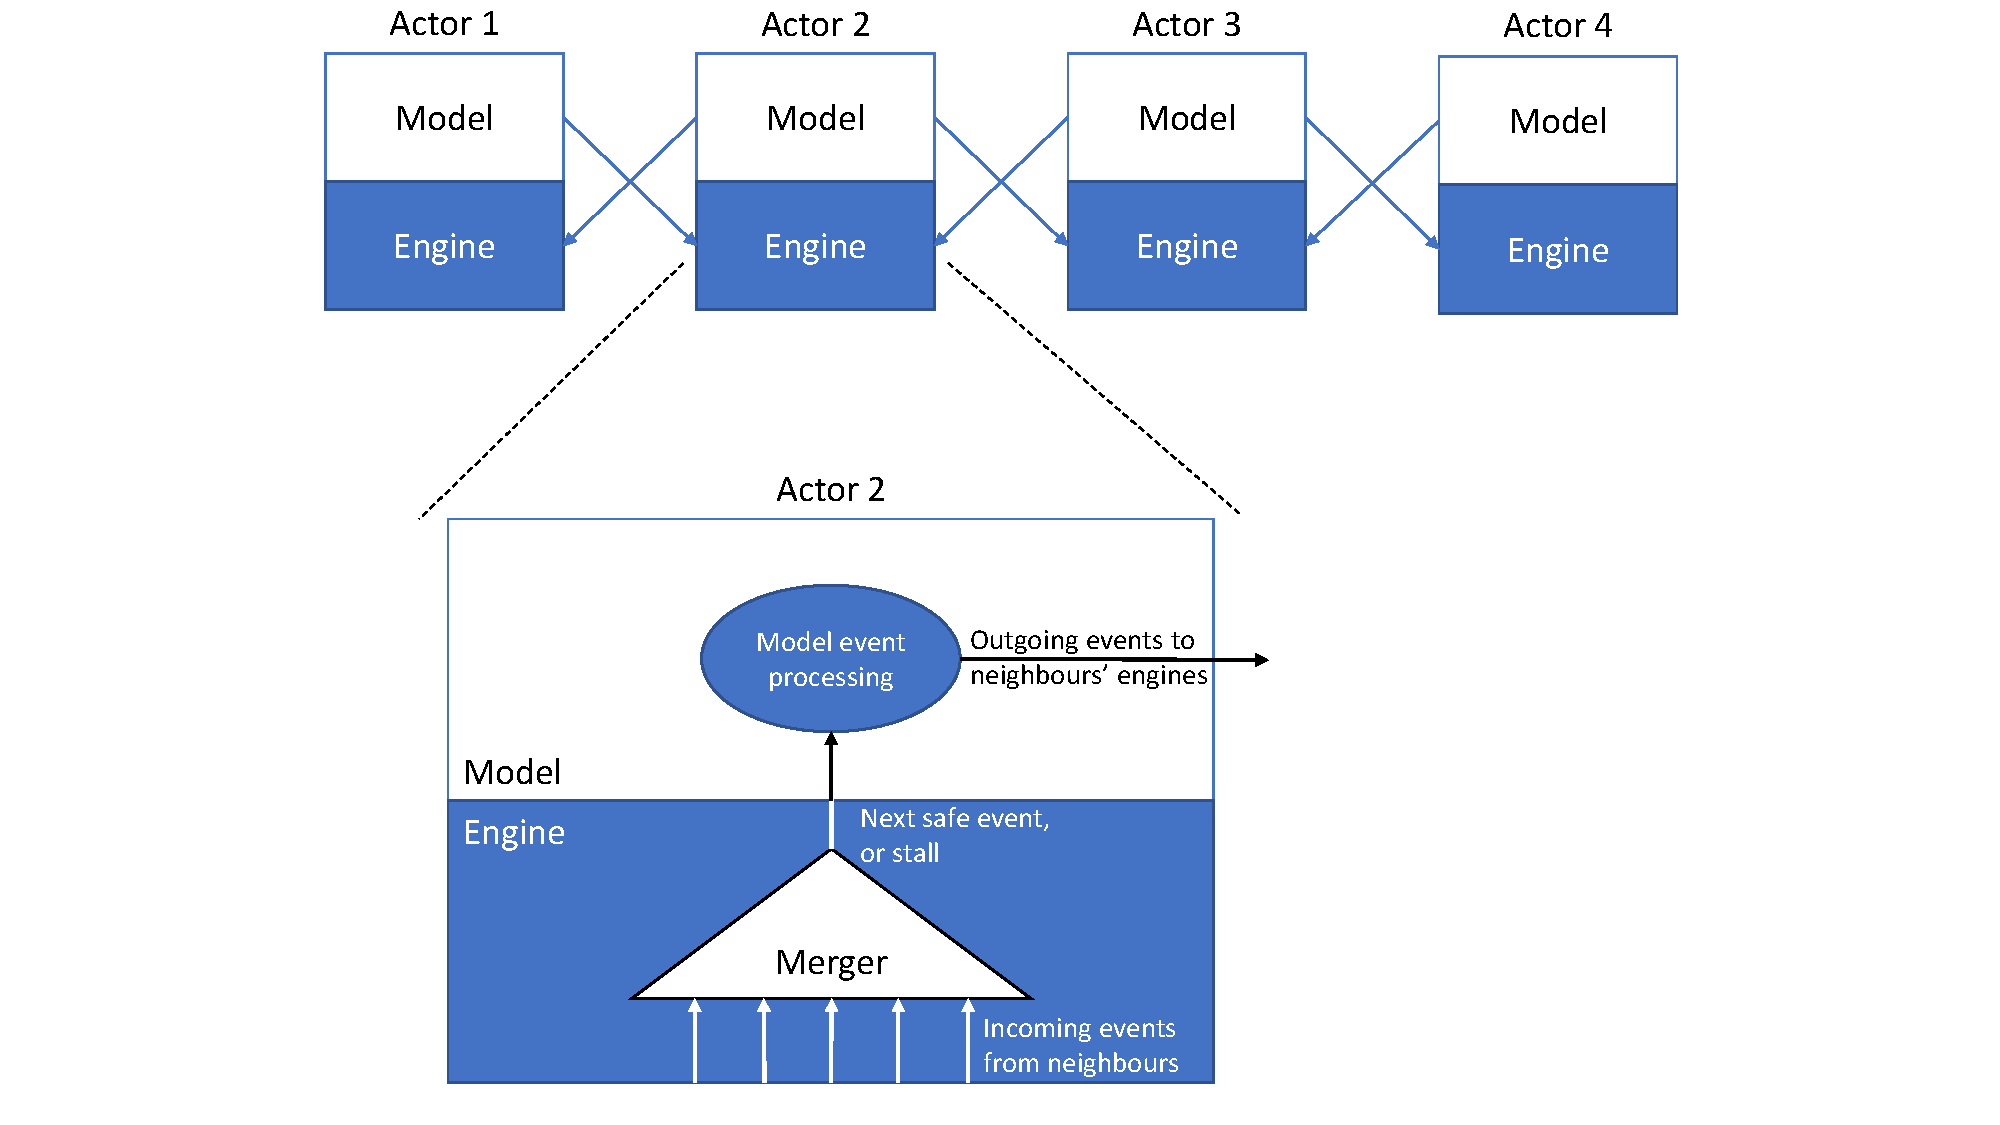
\includegraphics[width=\textwidth]{system-diagrams}
\caption{Rustasim actor overview. \manya{this figure is not mentioned in the text. point the reader to the figure where you are explaining the functionalities shown in the figure.}}
\end{figure}

A Rustasim simulation consists of many actors, each running concurrently, not necessarily simultaneously, to all others.
This concurrency brings with it all the challenges described in section\ \ref{pdes}: preserving causality and guaranteeing progress. \manya{if these two ended up being the most important challenges, then please mention them in the abstract and intro. }

To make developing models easier, Rustasim enforces a separation between the model and the code that deals with the parallel aspects of the simulation, the `engine'.
The engine and the model then have an application/system relationship: the engine receives all incoming events, arranges them in order and detects stall \manya{when do stalls happen? how common are they?}, returning to the user/model the events in order.
This abstraction very similar \manya{in general, the work "very" is redundant and should be omitted unless it's absolutely necessary to convey the message} to how applications interface with TCP: the application receives the bytes in-order while the OS handles the complexities of re-ordering and managing the connection.
The actor receives the events in order through an iterator, matches on the event type and executes the appropriate action.
It \manya{"it" refers to actor or engine?} is required to take certain actions upon receiving certain events.

Since there may be thousands or more of actors, \manya{for a data center simulation, what are the actors?} it is not possible to spin up separate threads for each of them.
Instead Rustasim spins up as many worker threads as there are available cores, and actors are scheduled on the workers.
The details of the scheduling are described in \ref{rustasim-sched}.



\subsubsection{The actor-engine abstraction} \label{rustasim-actor-engine}

The events in a distributed simulation are more complex than in a centralized one.
Although most events processed by actors are still model events, there is a need for additional event types in order to guarantee progress.\\
\code{Null} events are required to signal neighbours that it is safe for them to progress up to a certain time without waiting for this actor.
Without these messages, an actor cannot be sure if the silence from the neighbour comes from a lack of events to send, or from a delay in computation.
Although \code{Null} events are required to guarantee progress, actors will never receive them: they are only useful for the engine to progress, the actor need not take action on them.
The sole purpose of \code{Null} events is to allow the neighbours' engines to make progress.\\
Because the \code{Null} events require model-level knowledge to send \manya{unclear what sort of model-level knowledge is needed. please elaborate.}, the engine cannot do so on its own.
However, it is the engine that will become aware of a potential deadlock \manya{how?}, not the actor.
Therefore, to inform the actor of a potential stall, the engine generates a \code{Stalled} event \manya{which actor would receive the stalled event?}.
Upon receiving such an event, the actor is \emph{required} to send all necessary neighbours a \code{Null} event updating how far they may progress \manya{may or made?}.
If a neighbour has already received another event at, or past, the time the \code{Null} event would be received, the \code{Null} event is not sent. \manya{this whole para would be more clear if you could draw the state machine or decision tree for it. also a real simulation example would be great. something like this: consider two servers in a data center: A, B, C. Server A sends to B, etc. explain the events and how your actor-engine abstraction works in the example.}\\ %TODO make clearer
Finally, \code{Close} events tell the actor to return from its event loop.
Although this might seem trivial, it does require a little care, it is easy to leave the simulation hanging at this point. \manya{elaborate of the "care" part.}
It is necessary to also inform neighbours that we have no more events to communicate to them.
This can be done by sending \code{Null} events that pass closing times, or by sending \code{Close} events to the neighbours.

% TODO re-write, more details, reorgnize, cite?
\paragraph{Compiler enforcement}
By separating the actor and the engine into different crates, the modularity is strictly enforced by the Rust compiler, forbidding the simulator designer from modifying the internals of Rustasim.
In order to allow for arbitrary models to be built on top of Rustasim, the events that the engine deals with are parametrized through a generic type \code{T}.
Because the engine code is generic over \code{T}, it cannot make any assumptions about what the type looks like, lest the Rust compiler errors.
However, when compiled, the compiler will fill in the type appropriately and is able to optimize as though the type were written explicitly written in.\\
This separation between the model and the engine also allows for many different models to be implemented using the same engine, allowing for significant reuse between projects.
This is particularly appealing because most optimizations are implemented in the engine itself, and allowing further optimizations to be propagated to many simulations.
This separation also allows the writing of tests for the engine using a trivial model, making it easier to validate the engine and catch subtle errors.
\manya{at this point in the thesis, the simulator is described in abstract terms. somewhere in this chapter it would help to have a sample pseudocode with a simple topology as the front end of the simulator and show the inter-workings of the backend of the simulator to crystalize the functionality and modules.}

\subsection{Message passing} \label{rustasim-message-passing}

The communication between actors is done through a single-producer, single-consumer channel.
Rust offers a default channel implementation for multiple-producers and a single-consumer, which although technically correct isn't performant enough.
Multiple Rust crates offer more performant options, and after testing many different options, including Ringbuffer (TODO cite), crossbeam's (TODO cite) channels, the most performant option was the unreleased single-producer single-consumer queue from crossbeam.
In order to be easily published, Rustasim currently extracts the SPSC channel code from the unreleased branch of crossbeam.

\subsection{Multi-queue merging} \label{rustasim-tree}

This is the core of the engine: merging multiple queues together, and returning the next event if it has heard from all neighbours, as described in \ref{null-messages}.
If a neighbour has not been heard from, the scheduler should return a \code{Stalled} event.

\subsubsection{An initial approach: heaps}
An initial approach might be to maintain a heap of all received event along with a counter for the number of events in the heap from each sender.
The running time for this structure is sub-optimal, since it grows with to the amount of events in the queue, which is, due to the nature of waiting on everyone, always going to be nearly equal to, or greater than the number of neighbours.
The algorithmic complexity of processing or returning an event is then $O(\log e)$, with $e$ being the number of events in the queue.

An improved approach would take only the top event from each of the senders and maintain a heap of those.
The heap is then bounded by the number of senders, and the book-keeping is reduced to whether or not a sender has an element in the heap.
This structure then has an algorithmic complexity of $O\left(\log n\right)$
This works relatively well and does slightly improve running time.

When waiting on a neighbour, i.e. there are no events from at least one actor in the heap or in the incoming queue, the merger returns a \code{Stalled} event.
Otherwise, the merger returns the smallest current event off the heap, and attempts to extract an event from the incoming queue.
If there are no events in that neighbour's queue, the neighbour is marked as missing and the merger may stall when asked about the next event.

It is not necessarily true that marking a neighbour as missing results in a stall: it is possible that by the time the next event is requested from the merger, another event has been sent.
It is also possible that there is another event, from a different neighbour, that has the same time.
These tied events are all safe to return, and returning tied events can limit the number of stalls and increase performance.
This means that there may be more than one neighbour marked as missing without there being a stall.

\subsubsection{Loser trees}

Although there does not exist to my knowledge a structure with a better algorithmic performance, there exists structures with significantly better constant factors.
Notably, general purpose heaps can grow and shrink in size, and are non-monotonic: they do not require the input to be continuously growing to properly work.
By taking advantage of these two restrictions, we can reduce the complexity of the heap and dramatically increase the performance of the merger.
In some experiments, improvements can be greater than a factor of 2 over the heap.

Notably, this problem is essentially identical to the problem of merging tapes: there is a fixed number of tapes, and the reader cannot look ahead in the data, and we are required to assume the data on a single tape is already sorted.
Tournament trees in particular solve this problem elegantly.

A tournament tree takes in a certain number of elements to compare, here the next element of each of the queues and pairs them off.
The winner of each exchange, the event to be scheduled the soonest, moves on to fight another winner.
This process eventually forms a tree analogous to the structure of many tournaments.
Although it may be natural to record the winner of each exchange, recording the looser makes for a significantly more elegant algorithm as described by Knuth \cite{knuth_art_1998}.

\begin{figure}[h]
    \centering
    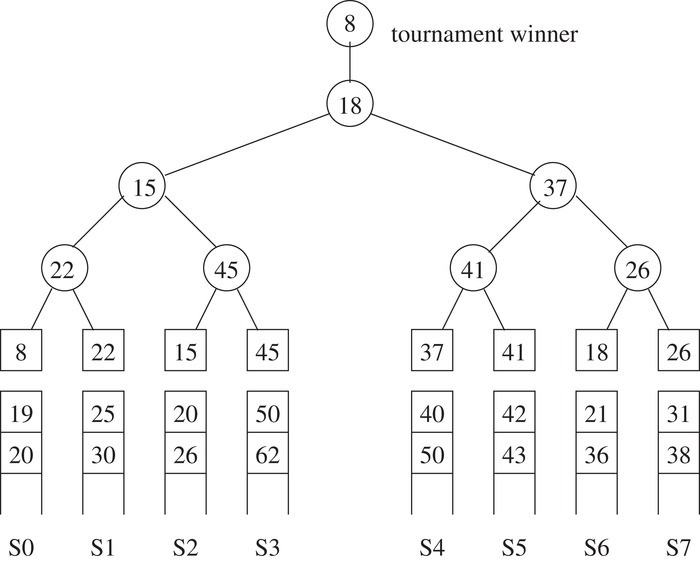
\includegraphics[width=\textwidth]{loser_tree}
    \caption{Loser tree example from TODO}
    \label{loser-tree:fig}
\end{figure}

In the example of Figure \ref{loser-tree:fig}, the current winner is 8, coming from \code{S0}.
In order to find the next smallest value, which a quick visual scan reveals should be 15 from \code{S2}, we re-run all the tournaments starting from \code{S0}.
The new value of \code{S0} is now 19, which goes up against the currently saved value in the parent: 22.
18 wins and moves on to go up against 15, which it loses.
Upon losing, we swap the two players, writing 18 down in the place of 15, and continuing 15 up the tree.
Reaching the root node of 18, current player 15 wins and is now the tournament winner.


\paragraph{Dealing with ties}
In order to allow tied events to be returned before a stall, when an incoming queue doesn't have any events to insert into the tree a \code{Stalled} event is inserted in its place.
The inserted event will then make its way to the top of the tree as though it were any other event, being returned when it is its time.
However, this alone doesn't mean all tied events will be returned, in order to guarantee that, \code{Stalled} events lose to events that are at the same time.

It is also important not to spuriously return a \code{Stalled} events: doing so will cause the actor to do expensive actions, and will upset the scheduling process described in \ref{rustasim-sched}.
When a \code{Stalled} event wins, the merger checks the neighbour's queue again and if it is no longer empty, will not return the \code{Stalled} event and will continue the process with the new event.


\subsection{Scheduling} \label{rustasim-sched}

\begin{figure}[h]
    \includegraphics[width=\textwidth,page=2]{system-diagrams}
    \caption{Rustasim actor overview}
    \label{rustasim-scheduling:fig}
\end{figure}

In the cases where there are less actors than available cores and there isn't contention on the system (no other CPU heavy job), it is possible to give each actor its own thread and still have excellent performance.
In this scenario when an actor stalls and is waiting on another, it can `busy-wait', burning CPU cycles until there is a new event on the channel.
More subtle synchronization primitives could be used, but all have some overhead, whereas checking in a tight loop has none.

However, The huge disadvantage of busy-waiting is that it gives the operating system no help as to which thread should be scheduled next, often scheduling threads that have nothing to do but burn cycles.
This issue alone is enough to make the simulator over 1,000x slower.
Explicitly yielding the thread on a stall sometimes improves the situation, but not much, since the OS still has no clear idea of who is best to schedule next.
In fact, cursory experiments suggest that it often repeatedly picks the same threads to schedule, letting it advance ahead of the rest, stall, and get rescheduled soon after, making little progress before stalling again, and so on.
Unfortunately switching between threads is an expensive operation for the operating system, and can easily take up a huge fraction of the simulation time.
In some runs, thread-switching took up almost two thirds of the simulation time, i.e. removing the scheduling issue could speed up the simulation by a factor of 3.
In addition to the overhead of thread switching, repeatedly stalling an operation sends out more \code{Null} events than necessary: they were not sent because of a deadlock, but because of a scheduling issue, creating overhead.
On its own, sending more events than needed may not seem like a big issue, they are cheap to process, but these \code{Null} events can become the main event type the stragglers receive, sometimes exceeding half of all received events.
\\


However, a better setup would be to have as many active actors as available cores, and to always schedule the most-straggling actor.
Indeed, being last means that the actor can run for longer uninterrupted, reducing the overhead of scheduling actors.

An easy way to schedule actors is such a pattern is to advance an actor until it stalls, then schedule every other actor, guaranteeing that the current actor is `last' before scheduling it again.

This can be done by having a single shared queue shared behind a lock, workers popping the front of the queue and pushing stalled actors at the back.
However, this queue then becomes a contention point between the actors.
This can be mitigated by having a few queues each with its own lock, and having workers randomly picking a queue and popping an event from it after pushing the stalled actor onto it.

\begin{figure}[h]
    \centering
    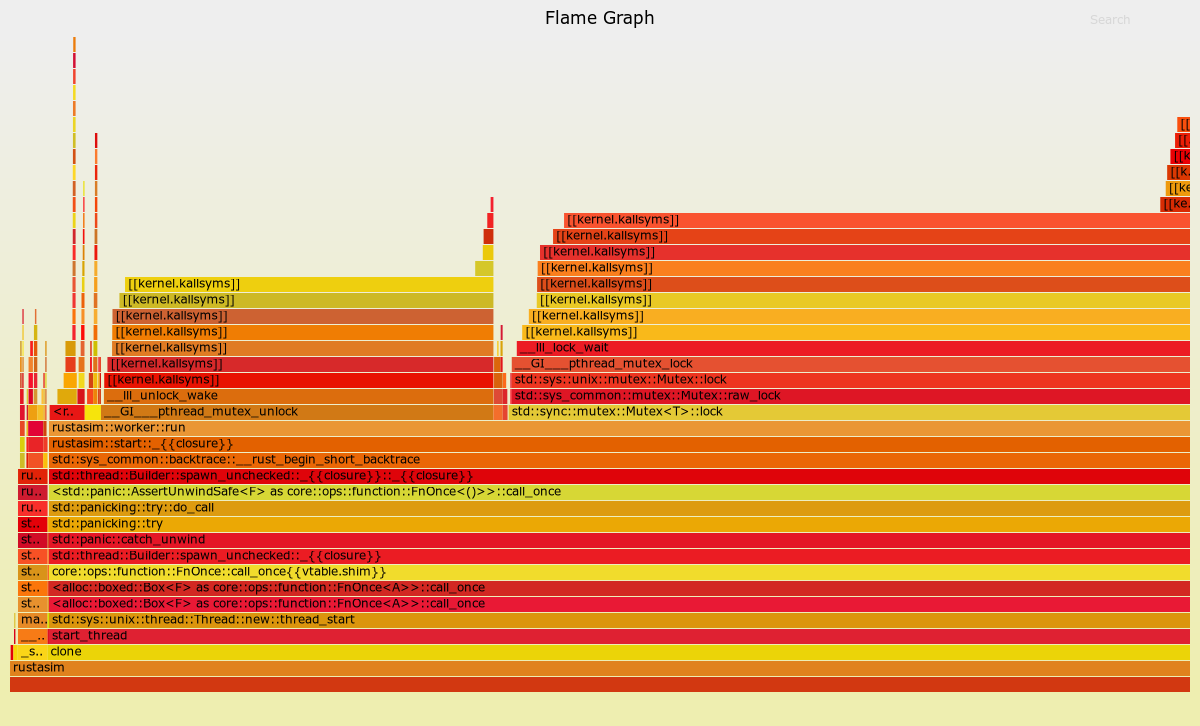
\includegraphics[width=\textwidth]{flame-lock-one-heap}
    \caption{`Flamegraph' of a Rustasim run with a single shared scheduling queue: lock contention accounts for over 90\% of the runtime.} %TODO cite
    \label{rustasim-lock-one-heap:fig}
\end{figure}

It is possible to push and pop from two distinct random queues, but this has the disadvantage of acquiring two locks for every scheduled actor and of allowing queues to drift to different sizes.
Pushing and popping from the same queue does not change the size of the picked queue since it both adds and removes an element from the queue before releasing it, and only acquires one lock.

Initializing and terminating the scheduler requires a little care: since the number of elements in the queues won't change size during the course of the program, they should all start with roughly the same number of actors each.
Failure to evenly distribute the queues may result in some actors being rescheduled too quickly or too slowly depending on if they end up in a shorter or longer queue, hurting performance.

Terminating the process is tricky: a single queue being empty indicates that some actors have finished, but does not indicate that all have.
In order to know when to terminate, a shared global counter is created which is incremented every time an actor finished.
When the shared counter reaches the number of actors, all actors are done and the workers can safely finish.
\\

In order to support this kind of scheduling, when actors are scheduled, they are required to only make progress as far as they can.
Once a \code{Stalled} event is received, they must return to let other actors be scheduled.
To allow the workers to distinguish a finished actor from a stalled actor, the actor returns either an \code{ActorState} which is either a \code{Continue(T)} containing the furthest time the actor got to, or a \code{Done(R)} containing the final result of the actor.
Although unused in this scheme, the furthest time reached by an actor can be used by more complex schedulers to further optimize the simulator's scheduling.

\subsection{Timeouts} \label{sim-timeouts}

Timeouts are by the nature of their generation, a little complicated to schedule in the simulator.
In order for an actor to send an event to itself, it must have itself as a neighbour.
In practice, this means that there is a queue whose receiving engine is the actor's own engine.

However, because timeouts can be generated for different values at different times, it is entirely possible for a timeout generated after a previous one to finish before the earlier one.
This out-of-order property means that we cannot simply use the event-merger to re-order the timeouts properly.
However, this can be solved by making use of the fact that timeouts have a large minimum value, a good fraction of a millisecond.

Instead of being sent to the actor, timeouts generated by a server are kept in a local heap, and a "check for timeout" event is sent to the engine.
Upon receiving the timeout, the server checks to see if any timeouts need to happen, and executes those.
The server also then schedules the next "check for timeout" event at that point.

Scheduling the "check for timeout" event is done by checking when the next timeout is scheduled to happen.
If the next timeout is going to happen sooner than any other timeout, i.e. it is scheduled to happen less than the mimimum timeout away, the checking event is scheduled for when the next timeout expires.
If the next timeout will expire longer than the minimum possible timeout in the future, the server schedules a check for a minimum timeout in the future: this will catch all fast timeouts which may generated before the current next timeout will expire.

Although this might seem slightly convoluted, this design for timeouts is efficient and highlights the flexibility of Rustasim in implementing patterns that may not seem to be part of its paradigm.


\subsection{Indexing} \label{rustasim-indexing}
% Not sure where this section best goes...

Although most programs consider the performance cost of a hash to be negligible, at the scale of nanoseconds, it becomes noticeable.
There is therefore a large incentive to not use hash tables and rely on the significantly faster direct indexing offered by arrays.
However, most data structures maintained by both the actor require indexing by the neighbour's \code{id}.
This \code{id} is unique across all actors and is useful for routing and for keeping track of who an event's sender is.

An alternative to structuring these data by \code{id} is to add every neighbour to an array and refer to them by their index.
Unfortunately that mapping isn't going to be regular across all actors, and some structure still explicitly require an \code{id}, notably packet destinations.

In order to minimize the amount of hashes to be made, each actor keeps track of a single hash table that maintains a translation from \code{ids} to an index \code{ix}, as well as an array containing an \code{ix} to \code{id} translation, mostly used for debugging purposes.
In addition, if the \code{id}s of all the devices in the network are continuous starting from 0, the routing table can be indexed, not hashed, by \code{id}, and return the appropriate index.

However, it is possible to avoid hash table lookups entirely with the cooperation of the engine.
The engine doesn't care about the model \code{id} of its neighbours, it only needs to receive its events.
By having the engine maintain the incoming queues in an array the same order as the actor has setup its \code{id}s, it is possible to translate the source \code{id} of the event to an index without needing a lookup.
Indeed, when the engine removes an event from a queue, it necessarily knows the index of that queue in its array of incoming queues.
It can then overwrite the incoming event's source field with the appropriate index, no lookup required.

Flows follow a similar pattern and are given a \code{flow\_id} only by the source server, akin to how TCP ports are used in the real world.
Each \code{flow\_id} can then simply be an index into an array, limiting the need for hash tables entirely.

The combination of these optimizations mean that there is almost no need to execute a hash table lookup in the normal processing of events.
The full translation tables, although never used in a proper simulation run, can be extremely helpful in debugging.

